\section{Results and discussion}
\label{sec:results}



\subsection{Synthetic gray-scale data}



\subsection{Simulated diffusion data}
%
The proposed method successfully reverted the synthetic distortion
field we applied to the data. With 16x16x16 control points, the
displacements field is dense enough to correctly represent the
synthetic field. (INCLUDE FIGURE). Figure XX shows the restored
image and a difference map with the original model (we can also
compute Dice indexes and that stuff).\\
%

\begin{figure}
\begin{tabular}{ccccc}
%\includegraphics[width=0.19\textwidth]{fig_modelFA_00} &
%\includegraphics[width=0.19\textwidth]{fig_modelFA_01} &
%\includegraphics[width=0.19\textwidth]{fig_modelFA_02} &
%\includegraphics[width=0.19\textwidth]{fig_modelFA_03} &
%\includegraphics[width=0.19\textwidth]{fig_modelFA_04} \\
%\includegraphics[width=0.19\textwidth]{fig_contours_00} &
%\includegraphics[width=0.19\textwidth]{fig_contours_01} &
%\includegraphics[width=0.19\textwidth]{fig_contours_02} &
%\includegraphics[width=0.19\textwidth]{fig_contours_03} &
%\includegraphics[width=0.19\textwidth]{fig_contours_04}
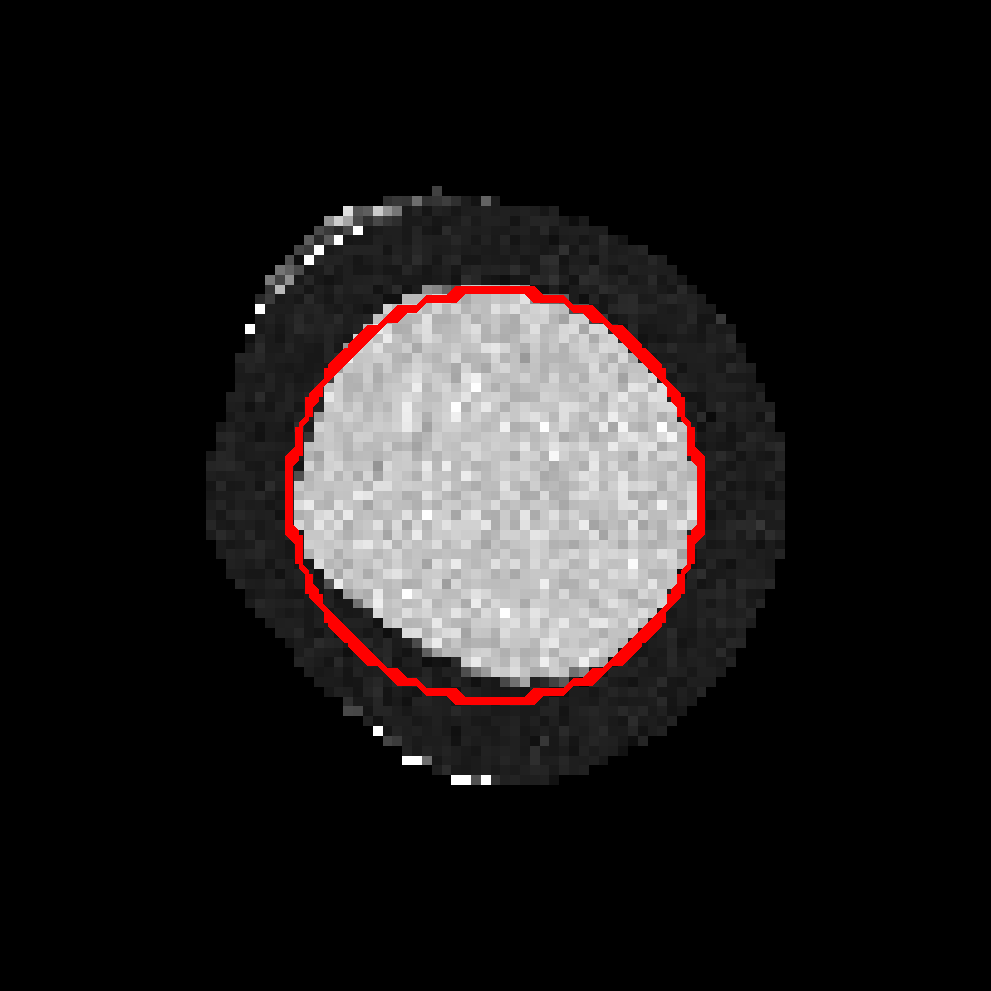
\includegraphics[width=0.19\textwidth]{model1result_b_1} &
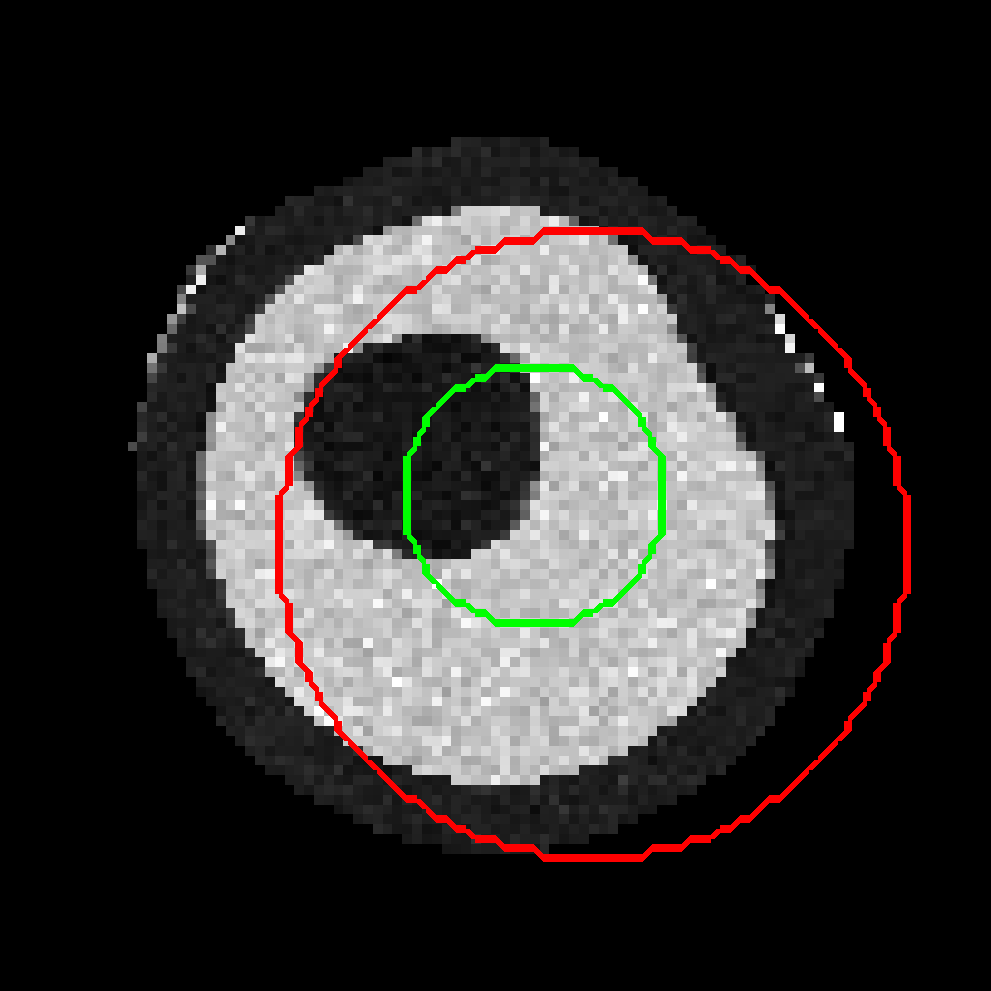
\includegraphics[width=0.19\textwidth]{model1result_b_2} &
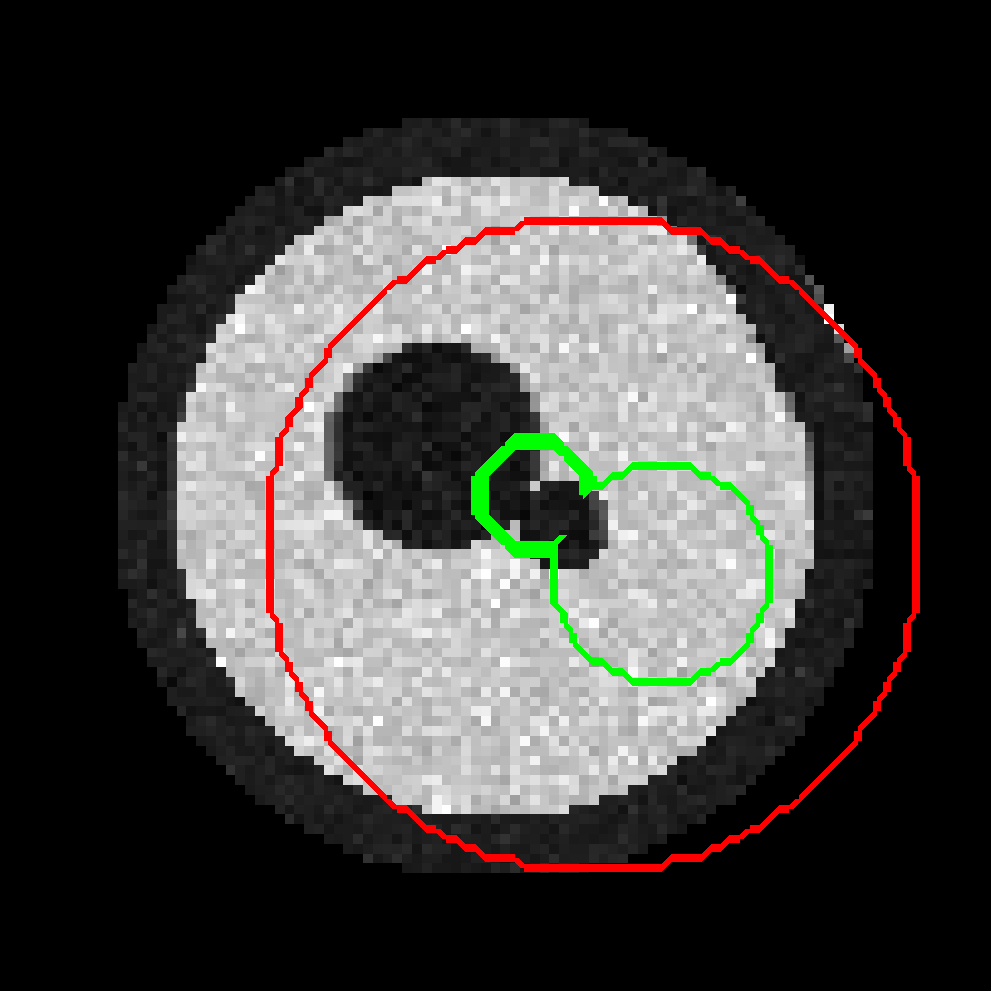
\includegraphics[width=0.19\textwidth]{model1result_b_3} &
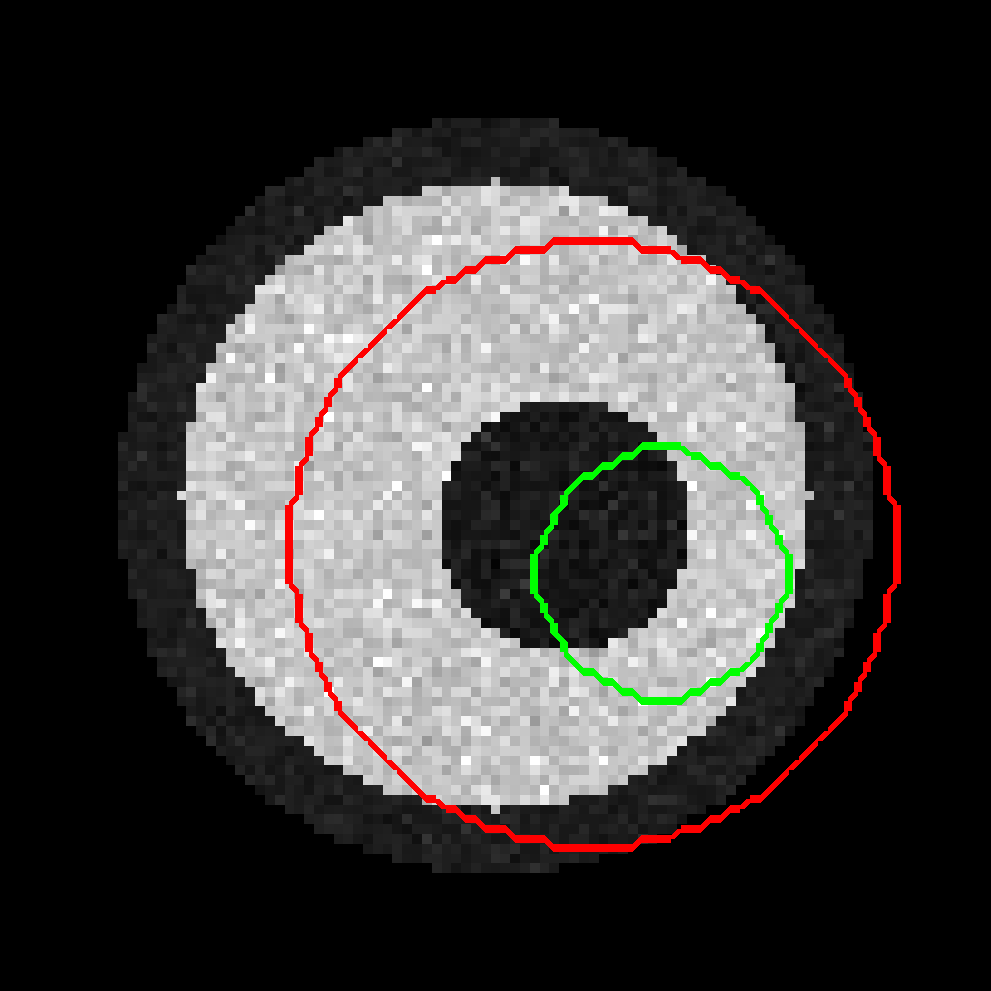
\includegraphics[width=0.19\textwidth]{model1result_b_4} &
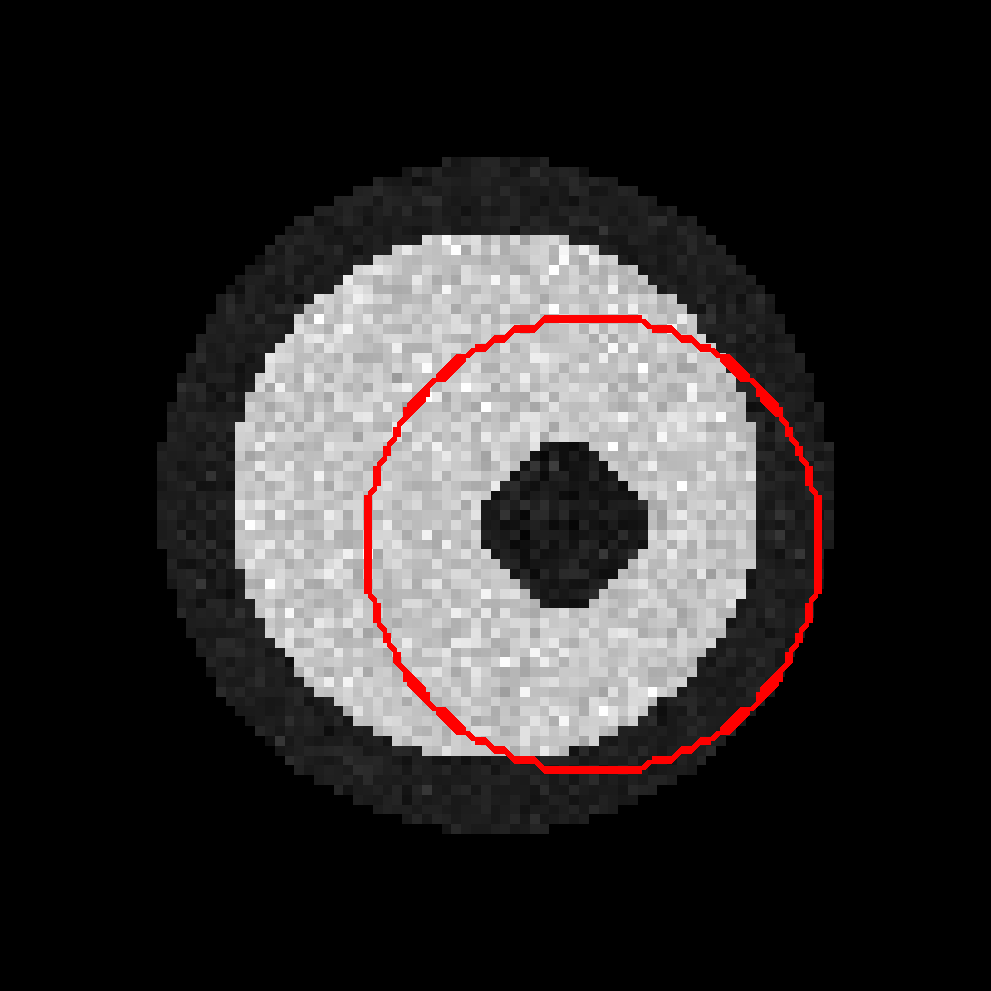
\includegraphics[width=0.19\textwidth]{model1result_b_5} \\
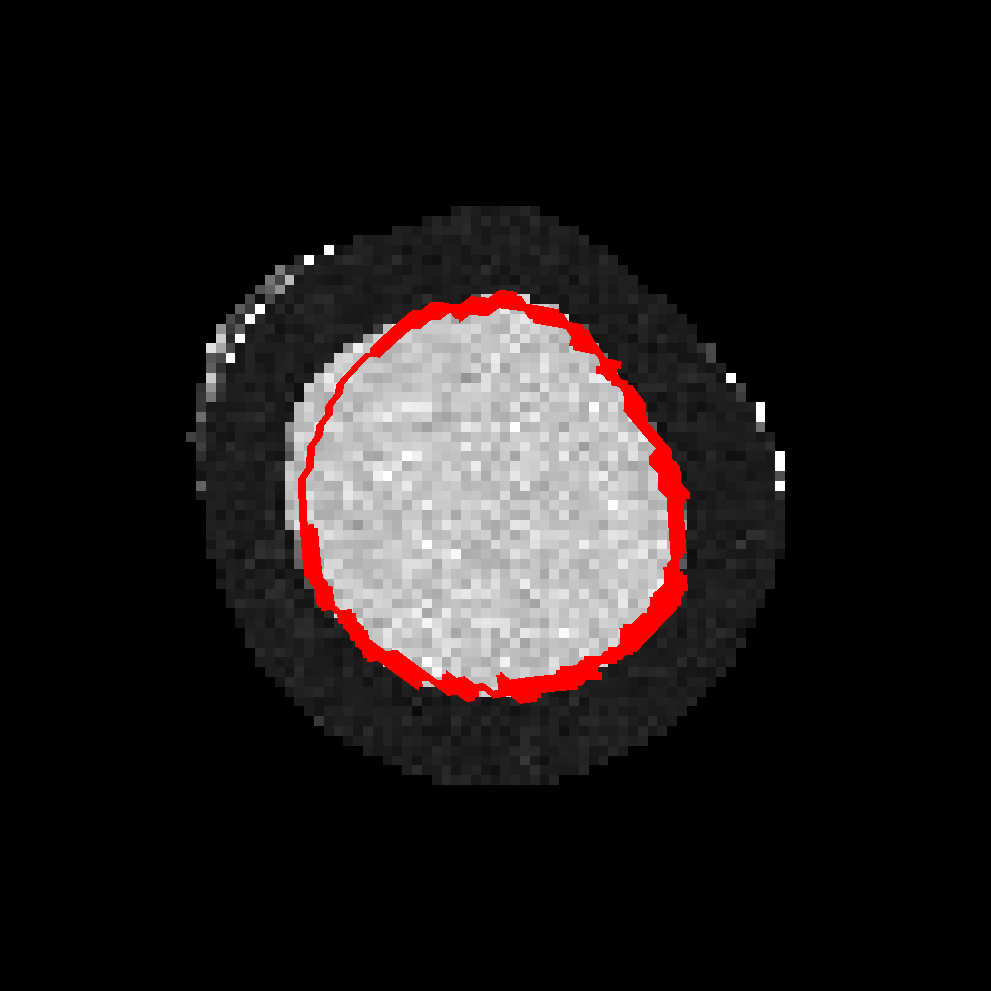
\includegraphics[width=0.19\textwidth]{model1result_a_1} &
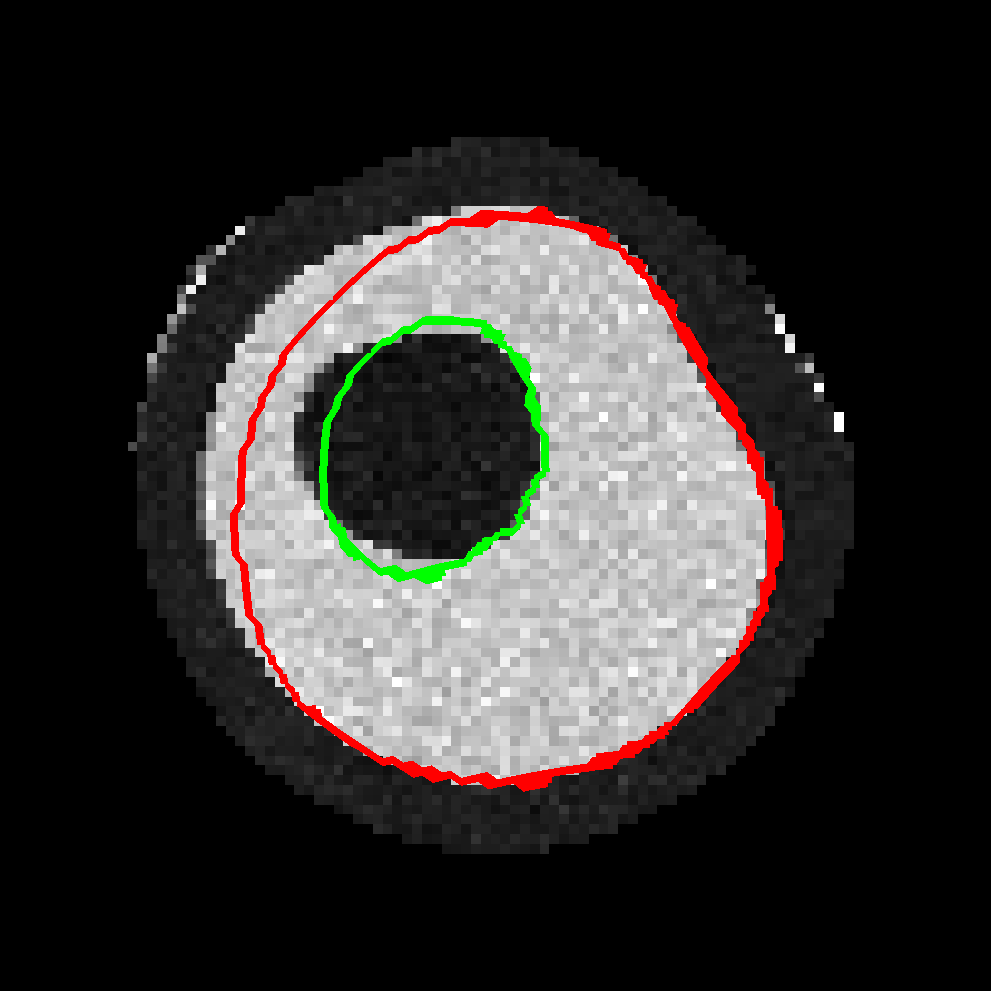
\includegraphics[width=0.19\textwidth]{model1result_a_2} &
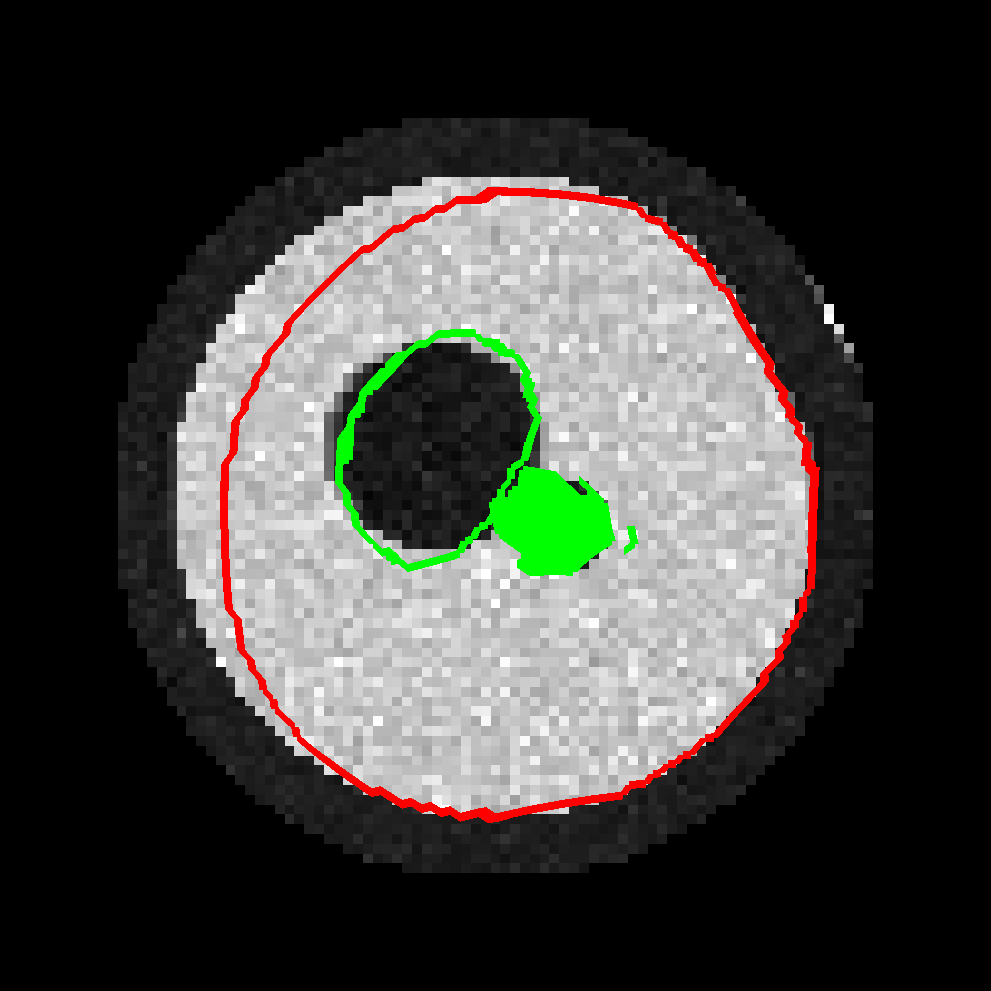
\includegraphics[width=0.19\textwidth]{model1result_a_3} &
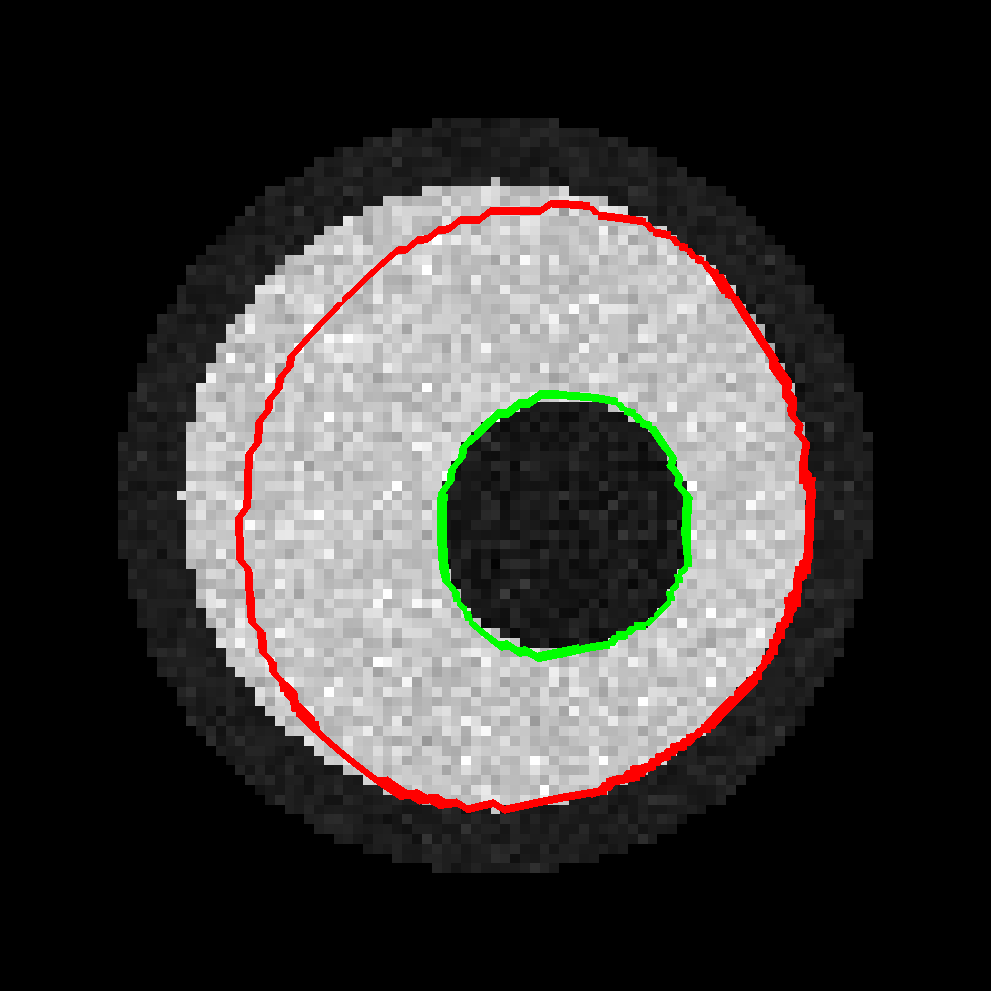
\includegraphics[width=0.19\textwidth]{model1result_a_4} &
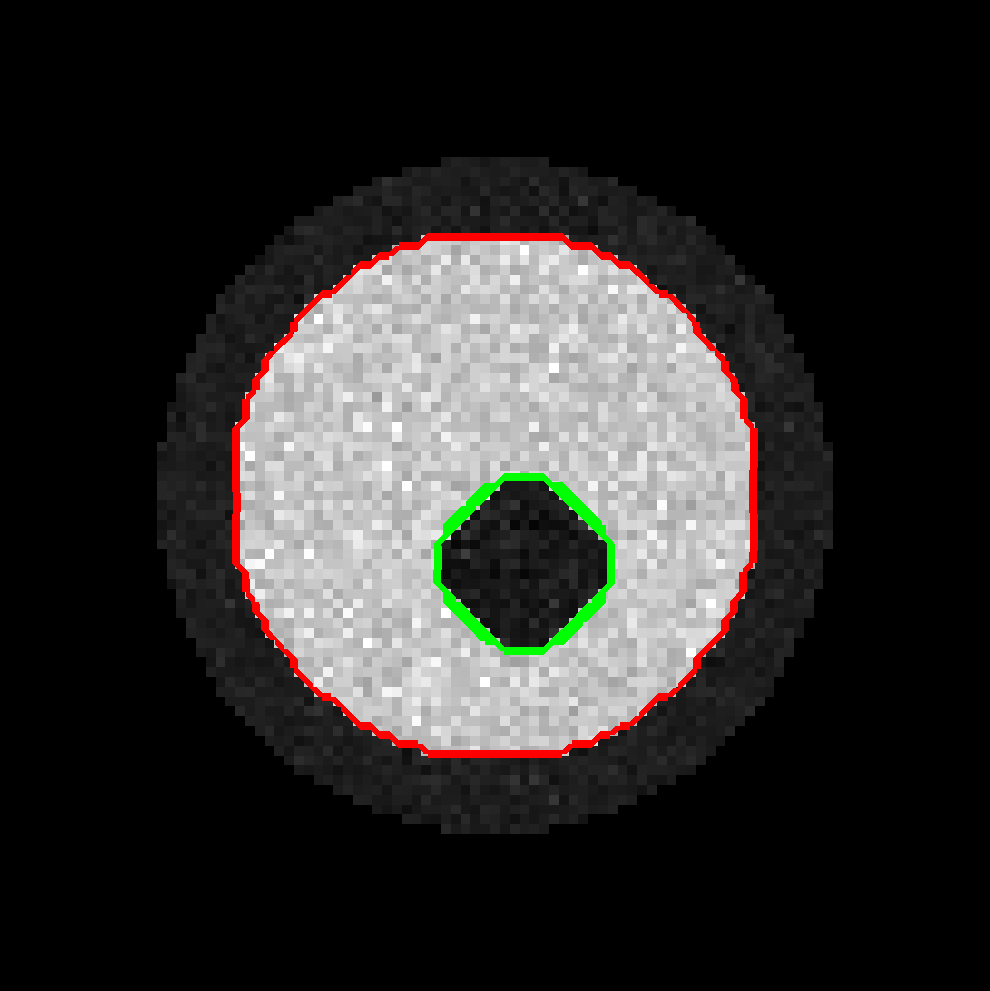
\includegraphics[width=0.19\textwidth]{model1result_a_5} \\
\end{tabular}
\caption{First row presents several slices along Z axis of the distorted \ac{fa} map and
the undistorted \ac{wm}-\ac{gm} and \ac{wm}-\ac{csf} contours given as shape priors. Second row contains the same map, now with the contours after joint segmentation-registration.}
\label{fig:fa}
\end{figure}